\documentclass[a4paper, 12pt]{article}
\usepackage{comment} % enables the use of multi-line comments (\ifx \fi) 
\usepackage{lipsum} %This package just generates Lorem Ipsum filler text. 
\usepackage{fullpage} % changes the margin
\usepackage{indentfirst}
\usepackage{graphicx}
\graphicspath{{./images/}}
\usepackage[colorlinks=true,linkcolor=black,urlcolor=cyan]{hyperref}

\begin{document}
%Header-Make sure you update this information!!!!
\noindent
\large\textbf{Understanding Git\footnote{\url{https://github.com/progit/progit2/releases/download/2.1.82/progit.pdf}}} \hfill \textbf{Filippo Cesaratto} \\
\normalsize

\section*{What is git?}
Git is a type of \textbf{version control system} (VCS) that makes it easier to track changes to files. For example, when you edit a file, git can help you determine exactly \emph{what} changed, \emph{who} changed it, and why.

It's useful for coordinating work among multiple people on a project, and for tracking progress over time by saving ``checkpoints''. 

\section*{The three states}
Each file in the \emph{working directory} can be in one of these two states: \emph{tracked} or \emph{untracked}. Tracked files are the files that git knows about. In fact these files had to be present in the last \emph{snapshot} git took, and can have one of these three possible states:
\paragraph{Committed/Unmodified} This means that the data is safely stored in your local database.
\paragraph{Modified} This means that you have changed your file, but have not committed it to your database yet. You have to use the command \textbf{add} to \emph{stage} it.
\paragraph{Staged} This means that you have marked a modified file in its current version to go into your next commit snapshot.

\vspace*{5mm}
\begin{figure}[h]
	\centering
	\includegraphics{FilesStates}
\end{figure}

\section*{Common commands}
Below is a series of basic commands with descriptions of what they each do.

\paragraph{git help $<$command$>$} This opens the browser and displays information about the given \textbf{command}. If a refresher is all that it's needed, just type: \textbf{git $<$command$>$ -h}.

\paragraph{git init}
This starts your own \emph{repository} from scratch in any existing directory on your computer. Git stores information about changes of the local (in the directory $D$ where git is initialized) files in a data structure called a \emph{repository}. This \emph{repository} is stored in a \emph{.git} directory inside the directory $D$ that is called the \emph{working directory}. No file of the directory $D$ is tracked yet.

\paragraph{git clone $<$URL$>$ [$<$directoryName$>$]}
This downloads an existing repository from the internet to your computer and extract the latest \emph{snapshot}. Almost all the files are downloaded so there is the possibility to open a previous snapshot of the downloaded project. By default it will be saved in the same directory where your repository is in, using the same name as the downloading snapshot, but if the optional parameter \textbf{directoryName} is given, then that would be its name.

\paragraph{git status}
This will print some basic information, such as which files have recently been modified. An option to shorten its content is \textbf{git status -s}.

\paragraph{git add $<$fileName$>$}
This adds \textbf{fileName} to the staged files that will be committed once the \textbf{commit} command is called. It's a multipurpose command: tracks new files, stages modified tracked files, and other things. Think as ``it adds precisely this content to the next commit''. There's the possibility of adding all the files in a directory; instead of inserting the file name, just insert the directory name in the \textbf{fileName} field. 

\paragraph{.gitignore}
This is not a command; it's a file in the root directory that git looks at to see if some of the files in that repository have to be shown (as \emph{untracked}) or not when calling the \textbf{status} command. A .gitignore file is a sequence of rules that prevent files to be looked at. An example (the text after the pound symbol is ignored):
\begin{verbatim}
	#ignore all .a files in this directory
	*.a
	#but do track lib.a, even though you're ignoring .a files above
	!lib.a
	#ignore TODO file in this directory
	/TODO
	#ignore all files in the build directory
	build/
	#ignore all the txt files in the subdirectory doc,
	#but not the subdirectory doc/server
	doc/*.txt
	#ignore all pdf files in doc and all its subdirectories
	doc/**/*.pdf	
\end{verbatim}

\paragraph{git diff} This lets you know what lines have been changed to a modified file since its last staging. This means the file was added to the stage files, and then edited. You can see the difference between what is going to be committed (\emph{staged} file) and the file as it is in this moment after the changing (\emph{modified} file). To compare the last commit (\emph{unmodified} file) to the staged changes (\emph{staged} file) the command is \textbf{git diff -{}-staged}. This doesn't look at the modified file that is not staged yet.

\paragraph{git commit} This commits all the \emph{staged} files. This means that those staged files and all the previously committed files (but not staged) will be inserted in a \emph{snapshot} of the project

\paragraph{git branch $<$newBranchName$>$}
This creates a local checkpoint technically called a \emph{reference} with the given \textbf{newBranchName}. A branch is an active line of development. The most recent commit on a branch is referred as the tip of that branch.

\paragraph{git checkout $<$existingBranchName$>$}


































\end{document}
